\documentclass{deliverablereport}

\deliverable{hpc}{singular-polyarith}
\deliverydate{30/08/2019}
\duedate{31/08/2019 (M48)}
\author{Daniel Schultz}

\usepackage[backend=bibtex]{biblatex}
\addbibresource{report.bib}

\usepackage{tikz}
\usetikzlibrary{plotmarks}

\begin{filecontents}{zp20.data}
#Threads 	Power [mW]
1	1.0
2	0.957696
3	0.958378
4	0.9413
6	0.947257
8	0.927686
10	0.904027
12	0.8998
14	0.911984
16	0.895612
20	0.860703
24	0.84717
28	0.847703
32  0.825368
\end{filecontents}

\begin{filecontents}{z20.data}
#Threads	Power [mW]
1	1.0
2	1.0
3	0.97561
4	0.955414
6	0.947867
8	0.931677
10	0.923077
12	0.917431
14	0.911854
16	0.903614
20	0.895522
24	0.892857
28  0.874636
32  0.765306
\end{filecontents}

\begin{filecontents}{zp20.data}
#Threads 	Power [mW]
1	1.0
2	0.957696
3	0.958378
4	0.9413
6	0.947257
8	0.927686
10	0.904027
12	0.8998
14	0.911984
16	0.895612
20	0.860703
24	0.84717
28	0.847703
32  0.825368
\end{filecontents}

\begin{filecontents}{z16.data}
#Threads	Power [mW]
1	1.0
2	0.94955
3	0.924561
4	0.89322
6	0.84051
8	0.823438
10	0.810769
12	0.80581
14	0.784226
16	0.765988
\end{filecontents}

\begin{filecontents}{zp16.data}
#Threads	Power [mW]
1	1.0
2	0.942149
3	0.924012
4	0.912
6	0.904762
8	0.904762
10	0.885437
12	0.883721
14	0.880309
16	0.863636
\end{filecontents}

\begin{document}
\maketitle
% This will be the abstract, fetched from the github description
\githubissuedescription
\clearpage
\tableofcontents

% write the report here

\section{Introduction}
\textsc{Singular} \cite{DGPS} represents polynomials as a linked list of terms in the sparse distributed format. For example, the polynomial $4 x^2 + 5 x y^2 z^3 + 6 y z^2$ with variables $x$, $y$, and $z$ might be stored as
\begin{center}
\begin{tabular}{ccc}
 & coefficient & exponents on ($x$,$y$,$z$)\\
term 1 & $4$ & $(2,0,0)$\\
term 2 & $5$ & $(1,2,3)$\\
term 3 & $6$ & $(0,1,2)$
\end{tabular},
\end{center}
where each term is essentially a coefficient together with an exponent tuple. This format is optimized for Gr\"obner basis calculations in algebraic geometry. However, because the terms themselves are stored in a link list, the \textsc{Singular} format is unsuitable for the arithmetic operations of multiplication, division, and greatest common divisor (GCD). For this reason \textsc{Singular} currently relies on the library \textsc{Factory} \cite{Factory} for these arithmetic operations. \textsc{Factory} is a self-contained {\tt c++} library for polynomial arithmetic that has been developed as part of \textsc{Singular}. Since the recursive representation in \textsc{Factory} is also not particularly well suited to parallelization, we have implemented for this deliverable \textsc{Singular}'s original sparse distributed format in the library \textsc{Flint} \cite{Hart2010}. \textsc{Flint} is a C library implementing basic arithmetic operations over a variety of coefficient domains and is already in direct use by \Sage for rational matrices and univariate polynomials. The implementation in \textsc{Flint} uses arrays, which means that the user has random access to the terms of their polynomials, and this is crucial for our parallel arithmetic operations.

The inclusion of \textsc{Flint} multivariate polynomial arithmetic has improved the single core performance of \textsc{Singular} on our set of benchmark problems by one to several orders of magnitude. \textsc{Singular} is one of the software components of \Sage used for multivariate arithmetic, so the users of \Sage will benefit seamlessly when the \textsc{Singular} version is updated. Since the \textsc{Flint} library itself is useful outside of \textsc{Singular}, we present the timings for the basic arithmetic operation in \textsc{Flint} as well as the timing of the operation in the new version of \textsc{Singular}, which includes all conversion and clean-up costs associated with \textsc{Singular}. As \textsc{Singular}'s main usage is as a Gr\"obner basis engine, it does not make sense to try to rewrite the polynomial format used natively by \textsc{Singular}. Instead, the conversion cost should be viewed simply as the time needed to convert polynomials to formats optimized for different purposes.

\section{Details of the systems}
Besides the three monomial orders \emph{lexicographic}, \emph{graded lexicographic} and \emph{graded reverse lexicographic} used commonly in \textsc{Singular}, \textsc{Flint} supports polynomials with exponents of unlimited size. Since \textsc{Singular} has a fixed and limited size on the exponents this second feature is somewhat moot for \textsc{Singular} users. About two years into this project we had to redesign the fundamentals of the multivariate polynomials in \textsc{Flint} to achieve the desired flexibility and performance. By the end of the next two years more than $100,000$ additional lines of code dedicated to multivariate arithmetic had been added. This includes many redesigns as bottlenecks were discovered and implementations were redone.

We run our benchmarks on the server {\tt nenepapa}, which has two sixteen core Intel Xeon E5-2697A v4 processors at $2.6$ GHz and $700$GB of memory. We show the timing of the basic operation in \textsc{FLINT} in the column labelled \emph{flint} and the timing of the new version of \textsc{Singular} in the column \emph{sing}. At the time of running these benchmarks, {\tt nenepapa} was also running two instances of long running calculations. This seemed to only slightly negatively affect the timings on $32$ threads.

The largest characteristic $p$ supported by \textsc{Singular} for arithmetic over finite fields is $p = 2^{29}-3$, and this is the prime we use to test arithmetic over $\mathbb{Z}/p \mathbb{Z}$. Both \textsc{Flint} and \textsc{Singular} use the \textsc{GMP} library for elements of $\mathbb{Z}$ with a special representation for integers less than $2^{62}$ ($2^{61}$ for \textsc{Singular}) in absolute value; small integers and elements of $\mathbb{Z}/p \mathbb{Z}$ both take one word of memory while large integers are managed by \textsc{GMP}. All times are reported in seconds.

Since these benchmarks deal with polynomials whose sizes are comparable to the total running time of the calculation, it is necessary to parallelize the conversion between \textsc{Flint} and \textsc{Singular}. This is a rather disappointing task as one direction is limited by the scaling of {\tt malloc} and the other direction is limited by \textsc{Singular}'s inherently serial data structure; the time to simply traverse \textsc{Singular}'s link list can be comparable to the time to do the threaded calculation in \textsc{Flint}. We encountered several performance quirks of {\tt malloc} on {\tt nenepapa}, which is running Gentoo Linux. The most noticeable of these was that, when constructing polynomials in \textsc{Singular}, the throughput of the {\tt malloc} provided by the system only starts to scale past $3$ or $4$ threads. Other implementations of {\tt malloc} such as {\tt tcmalloc} did not have this quirk but had overall higher times on $16$ threads. Therefore, we simply ran all of our benchmarks with the system's default {\tt malloc}. In order to use parallel conversion routines, the default allocator {\tt omalloc} of \textsc{Singular} must be disabled with the configuration option {\tt --disable-omalloc} as {\tt omalloc} is a special-purpose allocator that is not thread safe. Since this slows down the rest of \textsc{Singular} by about a factor of two, it may not be advantageous to disable {\tt omalloc} in practice. Nevertheless, we have disabled this to test the efficiency of the parallel conversion routines. 

We defined the efficiency on $n$ threads as
\begin{equation*}
\text{efficiency} = \frac{\text{ \textsc{Flint} time on $1$ thread}}{n \cdot \text{\textsc{Flint} time on $n$ threads}}\text{.}
\end{equation*}
In order to measure efficiency of the code, rather than the server CPU's, it is necessary to limit all CPU's to the same frequency, by disabling Intel's turbo boost, which otherwise runs the CPU at a higher frequency if fewer threads are being used (see Section \ref{section_code}). It is also necessary to pin threads to cores as {\tt nenepapa} is unable to consistently schedule threads on the same core and prefers hyperthreads over physical CPU's.

\section{Sparse Multiplication}
\label{section_sparse_mul}
Parallel multiplication has been investigated previously in \cite{Monagan:2009:PSP:1576702.1576739} and \cite{Gastineau:2013:HSM:2689622.2689630}. The more effective strategy for sparse polynomials is in the latter and seems to be the approach of directly calculating independent pieces of the answer. This makes the algorithm essentially lock-free, while the approach of \cite{Monagan:2009:PSP:1576702.1576739} requires a lock on its parallel merge. To test the effectiveness of this strategy, we time the multiplication $\cdot$ in
\begin{equation*}
(1+x+y+2z^2+3t^3+5u^5)^m \cdot (1+u+t+2z^2+3y^3+5x^5)^n
\end{equation*}
for $m=n=16$, where the product is already quite large with $28$ million terms. As shown in \cite{Monagan:2009:PSP:1576702.1576739}, it is difficult to obtain a good speed up on this example. The reason for this is that the inputs each have only $20$ thousand terms, so the majority of the time is spent writing down the answer, where only $14$ additions are done per term on average. Table \ref{table_sparse_mul1} shows the timings with $16$ threads. The poor scaling of the \textsc{Singular} times over $\mathbb{Z}$ can be explained easily: besides testing the multiplication in \textsc{Flint}, this benchmark tests the creation of large polynomials in \textsc{Singular}, which is a task bounded by the scaling of {\tt malloc}. In addition to having larger clean-up costs, the benchmark over $\mathbb{Z}$ puts three times as much pressure on {\tt malloc} as it does over $\mathbb{Z}/p\mathbb{Z}$.
\begin{table}[htb]
\begin{tabular}{l | r | r | r | r | }
 & \multicolumn{2}{|c|}{$\mathbb{Z}$} & \multicolumn{2}{|c|}{$\mathbb{Z}/p \mathbb{Z}$} \\ \hline
\#th   & flint & sing & flint & sing\\ \hline
$1$   & $10.54$ & $22.44$ &$9.12$ & $11.72$\\ \hline
$2$   & $5.55$  & $13.69$ &$4.84$ & $6.67$\\ \hline
$3$   & $3.80$  & $11.07$ &$3.29$ & $6.34$\\ \hline
$4$   & $2.95$  & $10.11$ &$2.50$ & $4.70$\\ \hline
$6$   & $2.09$  & $7.75$ &$1.68$  & $3.41$\\ \hline
$8$   & $1.60$  & $6.99$ &$1.26$  & $2.74$\\ \hline
$10$  & $1.30$  & $6.50$ &$1.03$  & $2.23$\\ \hline
$12$  & $1.09$  & $5.95$ &$0.86$  & $2.04$\\ \hline
$14$  & $0.96$  & $5.73$ &$0.74$  & $1.66$\\ \hline
$16$  & $0.86$  & $5.19$ &$0.66$  & $1.50$\\ \hline
\end{tabular}
\caption{Sparse multiplication for $(m, n) = (16, 16)$.}
\label{table_sparse_mul1}
\end{table}
The multiplication over $\mathbb{Z}/p \mathbb{Z}$ is overall faster and scales better. The efficiency on $16$ threads is $0.86$ versus an efficiency of $0.76$ over $\mathbb{Z}$. This is to be expected as the memory management of elements of $\mathbb{Z}$ via \textsc{GMP} adds overhead. As we increase the size of the problem we can observe better scaling as shown in Table \ref{table_sparse_mul2}. Now the efficiency on $16$ threads is $0.90$ ($0.90$ for $\mathbb{Z}/p \mathbb{Z}$), and the efficiency on $32$ threads is $0.76$ ($0.82$ for $\mathbb{Z}/p \mathbb{Z}$).
The efficiencies for all multiplications in this section are summarized in Figure \ref{figure_efficiencies}.
\begin{table}[htb]
\begin{tabular}{l | r | r | r | r | }
& \multicolumn{2}{|c|}{$\mathbb{Z}$} & \multicolumn{2}{|c|}{$\mathbb{Z}/p \mathbb{Z}$} \\ \hline
\#th   & flint & sing & flint & sing\\ \hline
$1$   & $120.0$ & $162.2$ &$53.88$ & $64.22$\\ \hline
$2$   & $60.0$ & $124.8$ &$28.13$ & $34.68$\\ \hline
$3$   & $41.0$ & $85.6$ &$18.74$ & $29.69$\\ \hline
$4$   & $31.4$ & $67.3$ &$14.31$ & $23.87$\\ \hline
$6$   & $21.1$ & $44.4$ &$9.48$ & $15.97$\\ \hline
$8$   & $16.1$ & $34.3$ &$7.26$ & $12.72$\\ \hline
$10$  & $13.0$ & $29.7$ &$5.96$ & $11.40$\\ \hline
$12$  & $10.9$ & $27.1$ &$4.99$ & $9.91$\\ \hline
$14$  & $9.4$ &  $25.2$  &$4.22$ & $9.00$\\ \hline
$16$  & $8.3$ &  $23.6$  &$3.76$ & $8.14$\\ \hline
$20$  & $6.7$ &  $21.5$  &$3.13$ & $7.16$\\ \hline
$24$  & $5.6$ &  $19.6$  &$2.65$ & $6.37$\\ \hline
$28$  & $4.9$ &  $18.8$  &$2.27$ & $5.62$\\ \hline
$32$  & $4.9$ &  $17.9$  &$2.04$ & $5.12$\\ \hline
\end{tabular}
\caption{Sparse multiplication for $(m, n) = (20, 20)$.}
\label{table_sparse_mul2}
\end{table}

\begin{figure}
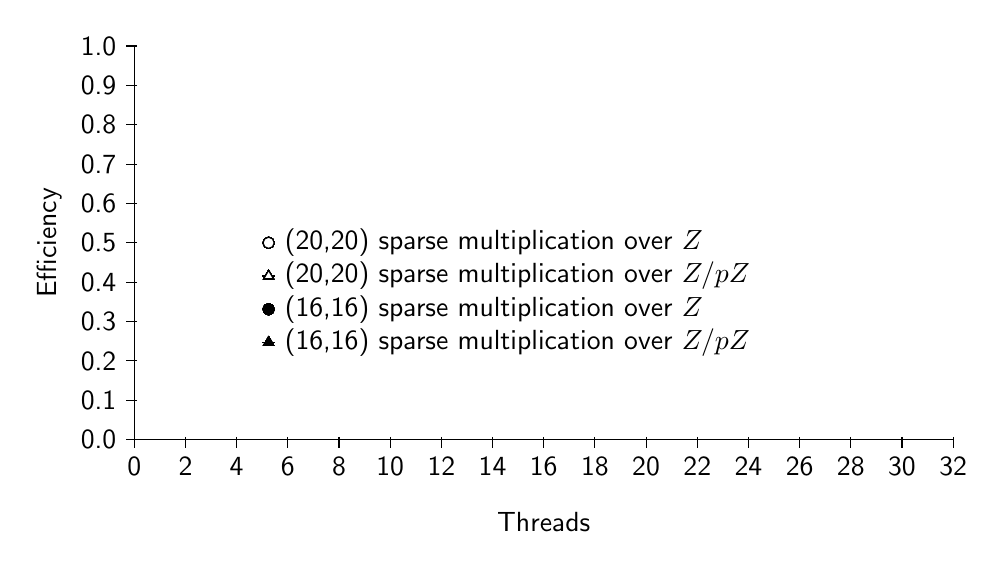
\begin{tikzpicture}[y=5cm, x=.325cm,font=\sffamily]
 	%axis
	\draw (0,0) -- coordinate (x axis mid) (32,0);
    	\draw (0,0) -- coordinate (y axis mid) (0,1);
    	%ticks
    	\foreach \x in {0,2,...,32}
     		\draw (\x,1pt) -- (\x,-3pt)
			node[anchor=north] {\x};
    	\foreach \y in {0.0,0.1,0.2,0.3,0.4,0.5,0.6,0.7,0.8,0.9,1.0}
     		\draw (1pt,\y) -- (-3pt,\y) 
     			node[anchor=east] {\y}; 
	%labels      
	\node[below=0.8cm] at (x axis mid) {Threads};
	\node[rotate=90, above=0.8cm] at (y axis mid) {Efficiency};

	%plots
	\draw plot[mark=*, mark options={fill=white}] 
		file {z20.data};
	\draw plot[mark=triangle*, mark options={fill=white} ] 
		file {zp20.data};
	\draw plot[mark=*, mark options={fill=black}] 
		file {z16.data};
	\draw plot[mark=triangle*, mark options={fill=black} ] 
		file {zp16.data};

    
	%legend
	\begin{scope}[shift={(5,0.5)}] 
	\draw[yshift=0\baselineskip] (0,0) -- 
		plot[mark=*, mark options={fill=white}] (0.25,0) -- (0.5,0) 
		node[right]{(20,20) sparse multiplication over $\mathbb{Z}$};
	\draw[yshift=-1\baselineskip] (0,0) -- 
		plot[mark=triangle*, mark options={fill=white}] (0.25,0) -- (0.5,0)
		node[right]{(20,20) sparse multiplication over $\mathbb{Z}/p\mathbb{Z}$};
	\draw[yshift=-2\baselineskip] (0,0) -- 
		plot[mark=*, mark options={fill=black}] (0.25,0) -- (0.5,0)
		node[right]{(16,16) sparse multiplication over $\mathbb{Z}$};
	\draw[yshift=-3\baselineskip] (0,0) -- 
		plot[mark=triangle*, mark options={fill=black}] (0.25,0) -- (0.5,0)
		node[right]{(16,16) sparse multiplication over $\mathbb{Z}/p\mathbb{Z}$};
	\end{scope}
\end{tikzpicture}
\caption{Efficiency of the sparse multiplication as defined by $\frac{\text{time on }1 \text{ thread}}{n \cdot \text{time on }n \text{ threads}}$}
\label{figure_efficiencies}
\end{figure}

\section{Dense Multiplication}
\label{section_dense_mul}
When the input polynomials have a density past a certain threshold, it is possible to do better than algorithms based on heaps. For this reason we implemented an approach based on arrays and parallelized it. The approach is suited well to the multiplication in, for example,
\begin{equation*}
(1+x+y+z+t)^m \cdot (1+x+y+z+t)^n\text{,}
\end{equation*}
As the inputs to the multiplication in this case each have $46$ thousand terms, and the product only has $635$ thousand terms, the amount of work per output term is much higher than in Section \ref{section_sparse_mul}. Table \ref{table_dense_mul} shows that the efficiency on $16$ threads is $0.93$ in both cases. However, as this approach breaks up the input problem into a limited number of pieces, and only some of these pieces are large, this approach is effective at low thread counts but does not scale past $16$ threads. 

\begin{table}[htb]
\begin{tabular}{l | r | r | r | r | }
& \multicolumn{2}{|c|}{$\mathbb{Z}$} & \multicolumn{2}{|c|}{$\mathbb{Z}/p \mathbb{Z}$} \\ \hline
\#th   & flint & sing & flint & sing\\ \hline
$1$   & $5.08$ & $5.39$ &$3.64$ & $3.71$\\ \hline
$2$   & $2.56$ & $2.80$ &$1.83$ & $1.90$\\ \hline
$3$   & $1.71$ & $1.90$ &$1.22$ & $1.28$\\ \hline
$4$   & $1.29$ & $1.45$ &$0.92$ & $0.98$\\ \hline
$6$   & $0.86$ & $1.00$ &$0.62$ & $0.66$\\ \hline
$8$   & $0.67$ & $0.77$ &$0.46$ & $0.50$\\ \hline
$10$  & $0.52$ & $0.63$ &$0.37$ & $0.40$\\ \hline
$12$  & $0.46$ & $0.55$ &$0.31$ & $0.34$\\ \hline
$14$  & $0.40$ & $0.50$ &$0.28$ & $0.30$\\ \hline
$16$  & $0.34$ & $0.43$ &$0.24$ & $0.26$\\ \hline
\end{tabular}
\caption{Dense multiplication for $(m, n) = (30, 30)$.}
\label{table_dense_mul}
\end{table}

\section{Sparse Division}
For this benchmark we simply divide the product in Section \ref{section_sparse_mul} by the divisor $(1+u+t+2z^2+3y^3+5x^5)^n$.
It is important to note that we are in fact computing two things: (1) whether the dividend is divisible by the divisor and (2) the quotient if it is. As with sparse multiplication, the approach of Gastineau and Laskar \cite{Gastineau:2015:PSM:2790282.2790285} scales better than the approach of Monagan and Pearce \cite{Monagan:2010:PSP:1837210.1837227}. Division is more difficult to parallelize than multiplication because the algorithm is highly sequential: Most terms in the quotient depend on previous terms in the quotient for their calculation. For this reason, the algorithm requires locks on the generated quotient, and only one thread can be generating quotient terms at a time. We achieve an efficiency of $0.71$ on $16$ threads ($0.78$ for $\mathbb{Z}/p\mathbb{Z}$) as shown in Table \ref{table_sparse_div}.
Since one of the inputs to the algorithm is large, this tests not only the division in \textsc{Flint} but also the conversion from \textsc{Singular} to \textsc{Flint}. In order to obtain reasonable timings with \textsc{Singular} over $\mathbb{Z}$, it was necessary to force \textsc{Flint} to borrow \textsc{Singular}'s integers. With this optimization the overhead over $\mathbb{Z}$ is much less than the corresponding overhead in Table \ref{table_sparse_mul1}. However, conversion overhead does not scale well for the following reason: The time to merely traverse \textsc{Singular}'s linked list representation of the dividend is about $0.7$ seconds in this benchmark. This operation is necessary to find the polynomial's length, is an inherently serial operation, and consumes all of the conversion overhead over $\mathbb{Z}/p\mathbb{Z}$ on $16$ threads.

\begin{table}[htb]
\begin{tabular}{l | r | r | r | r | }
 & \multicolumn{2}{|c|}{$\mathbb{Z}$} & \multicolumn{2}{|c|}{$\mathbb{Z}/p \mathbb{Z}$} \\ \hline
\#th   & flint & sing & flint & sing\\ \hline
$1$   & $9.96$ & $13.29$ &$9.60$ & $11.44$\\ \hline
$2$   & $5.22$ & $7.48$ &$4.74$ & $5.82$\\ \hline
$3$   & $3.64$ & $5.75$  &$3.31$ & $4.15$\\ \hline
$4$   & $2.68$ & $4.66$  &$2.54$ & $3.17$\\ \hline
$6$   & $1.92$ & $3.50$  &$1.68$ & $2.80$\\ \hline
$8$   & $1.55$ & $2.93$  &$1.34$ & $2.06$\\ \hline
$10$  & $1.26$ & $2.76$  &$1.17$ & $1.82$\\ \hline
$12$  & $1.14$ & $2.54$  &$1.03$ & $1.57$\\ \hline
$14$  & $0.92$ & $2.30$  &$0.90$ & $1.44$\\ \hline
$16$  & $0.88$ & $2.01$  &$0.78$ & $1.30$\\ \hline
\end{tabular}
\caption{Sparse division for $(m, n) = (16, 16)$.}
\label{table_sparse_div}
\end{table}

\section{Sparse GCD}
For this benchmark we calculate $\operatorname{gcd}(a^{m_1}b^{n_1}, a^{m_2}b^{n_2})$\text{,}
where $a=1+x+y^5+z^4+t^{40}+u^{50}$ and $b=1+x^9+y^2+z^{11}+t^7+u^{27}$. This calculation requires at least a dozen steps to be completed in serial, and we achieve an efficiency of $0.72$ on $16$ threads ($0.66$ for $\mathbb{Z}/p\mathbb{Z}$) by parallelizing the majority of these steps as shown in Table \ref{table_sparse_gcd}. The overhead from converting between the \textsc{Singular} format is negligible here. The algorithm over $\mathbb{Z}/p\mathbb{Z}$ suffers because, while the input problem can be split up into several pieces of work, the recombination of the results from each thread is an extra step not present in the serial algorithm. Furthermore, this recombination becomes less efficient with greater numbers of smaller pieces.
\begin{table}[htb]
\begin{tabular}{l | r | r | }
 & $\mathbb{Z}$ & $\mathbb{Z}/p \mathbb{Z}$ \\ \hline
\#th   & flint & flint\\ \hline
$1$   & $23.24$ & $117.8$ \\ \hline
$2$   & $12.26$ & $59.8$ \\ \hline
$3$   & $8.24$  & $42.5$ \\ \hline
$4$   & $6.26$  & $32.2$ \\ \hline
$6$   & $4.41$  & $24.2$ \\ \hline
$8$   & $3.42$  & $17.6$ \\ \hline
$10$  & $2.87$  & $15.6$ \\ \hline
$12$  & $2.50$  & $13.4$ \\ \hline
$14$  & $2.23$  & $11.3$ \\ \hline
$16$  & $2.03$  & $11.2$ \\ \hline
\end{tabular}
\caption{Sparse GCD for $(m_1, n_1) = (8, 5)$, $(m_2, n_2) = (3, 9)$.}
\label{table_sparse_gcd}
\end{table}

\section{Dissemination and impact}

This project has been the topic of an extensive blog \url{http://wbhart.blogspot.com/2019/08/parallel-multivariate-arithmetic-final.html}. The linked article was read by over 200 individuals and was noticed by all of the leading experts in parallel polynomial arithmetic, whom we have been in constant contact with.

A Jupyter notebook demonstrating our code running is available at \url{https://github.com/tthsqe12/SingularParallelArithmetic}.

It is worth pointing out some of the ways in which we and others have and will benefit from this work, and what are some of the hard restrictions.

There are four main areas where fast polynomial arithmetic can be expected to speed up important research applications using Singular. We will discuss each in turn.

\begin{enumerate}
\item Basic arithmetic for arithmetic's sake.
\item Gr\"{o}bner bases.
\item Primary decomposition/factorisation.
\item Rational functions.
\end{enumerate}

No. 1. Here we are talking about users implementing algorithms in Singular which need to do basic arithmetic, i.e. multiplication, division and gcd of polynomials. As the default polynomial format in Singular is the linked-list sparse distributed format, a conversion to and from Flint array sparse distributed format is unavoidable. One still gets a big speedup in practice, but as you can see from timings, conversion costs may actually dominate, meaning you don't get a linear speedup with cores. This is essential behaviour and we have expended much effort in minimizing the cost. The user still wins, however, so it is worth the effort. The timings above directly demonstrate these benefits.

No. 2. Here you can only expect to gain when there are large divisions done in the Buchberger algorithm for Gr\"{o}bner bases, which is not used for every Gr\"{o}bner basis application. However, it does still have significant applications. We have encountered such examples in real world applications recently (albeit with orderings that we nearly but don't quite support yet). Many such examples exist in real research with orderings that we do support and we expect big gains here. Work under this heading (supporting additional orderings, etc.) will go on for years after ODK and we will be leveraging the new multivariate engine in many new ways.

No. 3. Primary decomposition depends heavily on factorisation of multivariate polynomials. But factorisation can be a life's work, compared to a four year ODK project, and so lies completely outside the scope of ODK. Daniel Schultz has already begun work on integrating the ODK parallel multivariate work in the Singular factoring engine, as a means of disseminating our work, and the preliminary results are extremely encouraging.

No. 4. William Hart and Hans Sch\"{o}nemann have been implementing fast rational functions based on the ODK work. Here conversion costs do NOT occur. Rational functions are constructed in the Flint array format and never leave that format. One can even do Gr\"{o}bner bases over rational function fields without conversion, and this is a very important application in Singular. However, one should temper one's expectations. Although the single core gains may make orders of magnitude difference here, it is common for the rational functions to be too small to benefit from parallelisation. However, when "coefficient explosion" does occur, then it becomes critical. However, one should also realise that in such cases it is often better to use a modular Gr\"{o}bner basis algorithm, if available. On the other hand, this may have been merely due to the prior lack of fast rational functions in the past, and even with the modular algorithm, one will still critically benefit from the ODK work, since one still has to do the same computations mod p, which our ODK work implements. The code for fast rational functions is currently essentially finished (it has been written by William Hart, independently of ODK funding but directly based on the fast ODK arithmetic). It needs some new Singular interpreter features to be added by Hans Sch\"{o}nemann when he returns from holidays in order to be functional. Experience tells us the speedups could potentially be orders of magnitude (seconds compared to weeks in some real world cases).

We should also mention that the new computer algebra system Oscar is already benefiting from the ODK work. For example, Oscar depends on the ODK work entirely for an important application from group theory (again using fast rational functions). There are also already applications in number theory within our research group in Kaiserslautern. That's all completely independent of ODK, but it's worth knowing that the benefits are being multiplied across multiple systems.

From an Oscar perspective, the conversion costs mentioned above are only incurred when converting \emph{from} the Flint format \emph{to} Singular format when a Groebner basis computation is needed, where the conversion cost is usually not relevant compared to the cost of the Groebner basis computation, which can be doubly exponential (in the worst case). Other systems are free to approach things in a similar way, and then the cost of conversion becomes a moot point. We have in fact learned a lot about how such a system should be constructed from this work, which we look forward to sharing with the community, both through our ODK dissemination and ongoing research projects.

\section{Comparisons with other systems}
\subsection{Giac}
\textsc{Giac} \cite{Giac} is a computer algebra kernel used in many
well-known symbolic systems and calculators. At the time of writing,
we were unable to install \textsc{Giac} on our Gentoo server with all
its optimizations enabled. Updates from the author will be provided
on the aforementioned blog.

\subsection{Trip}
\textsc{Trip} \cite{Gastineau:2011:TCA:1940475.1940518} is a system dedicated to computations in celestial mechanics and offers parallel polynomial multiplication over $\mathbb{Z}$ in a variety of polynomial formats. We chose the format that seemed to give the best timings on {\tt nenepapa}. We noted that version 1.6.42 of \textsc{Trip} suffered from poor scalability. One of the authors pointed out that this is due to usage of the system {\tt malloc} and provided us with a patched version of \textsc{Trip} using {\tt jemalloc} and instructions to test it over $\mathbb{Z}/p\mathbb{Z}$. It is interesting to note that \textsc{Trip} reaches an efficiency of $0.82$ on our largest benchmark for \emph{both} $\mathbb{Z}$ and $\mathbb{Z}/p\mathbb{Z}$, suggesting that it handles elements of $\mathbb{Z}$ with slightly better scaling than \textsc{Flint}.
\begin{table}[htb]
\begin{tabular}{l | r | r | r | r | r | r | r | r | r |}
 & \multicolumn{3}{|c|}{\textsc{Trip}} & \multicolumn{6}{|c|}{\textsc{Trip} patched} \\ \hline
 & {dense} & \multicolumn{2}{|c|}{sparse} & \multicolumn{2}{|c|}{dense} & \multicolumn{4}{|c|}{sparse} \\ \hline
\#th  & $(30, 30)$ & $(16, 16)$ & $(20, 20)$ & \multicolumn{2}{|c|}{$(30, 30)$} & \multicolumn{2}{|c|}{$(16, 16)$} & \multicolumn{2}{|c|}{$(20, 20)$}\\ \hline
 & $\mathbb{Z}$ & $\mathbb{Z}$ & $\mathbb{Z}$ & $\mathbb{Z}$ & $\mathbb{Z}/p\mathbb{Z}$ & $\mathbb{Z}$ & $\mathbb{Z}/p\mathbb{Z}$ & $\mathbb{Z}$ & $\mathbb{Z}/p\mathbb{Z}$ \\ \hline
$1$   & $24.40$ & $21.90$ & $130.00$ &  $25.61$ & $30.55$ & $24.01$ & $27.94$ & $140.10$ & $175.10$\\ \hline
$2$   & $12.30$ & $11.50$ & $67.2$   &  $12.78$ & $15.31$ & $11.92$ & $14.01$ & $69.86$ & $87.47$\\ \hline
$3$   & $8.30$ & $8.02$  & $45.7$    &  $8.55$ & $10.21$ & $8.06$ & $9.38$ & $46.74$ & $59.11$\\ \hline
$4$   & $6.21$ & $6.02$ & $33.4$     &  $6.44$ & $7.65$ & $6.13$ & $7.18$ & $35.24$ & $48.51$\\ \hline
$6$   & $4.24$ & $3.96$ & $22.9$     &  $4.38$ & $5.21$ & $4.19$ & $5.14$ & $25.02$ & $31.78$\\ \hline
$8$   & $3.17$ & $3.29$ & $17.3$     &  $3.36$ & $3.97$ & $3.19$ & $3.80$ & $18.70$ & $23.31$\\ \hline
$10$  & $2.87$ & $2.68$ & $15.5$     &  $2.81$ & $3.17$ & $2.60$ & $3.02$ & $15.06$ & $18.97$\\ \hline
$12$  & $2.47$ & $2.30$ & $12.9$     &  $2.34$ & $2.86$ & $2.19$ & $2.60$ & $12.62$ & $15.60$\\ \hline
$14$  & $2.01$ & $2.07$  & $11.0$    &  $1.98$ & $2.50$ & $1.99$ & $2.25$ & $10.80$ & $13.55$\\ \hline
$16$  & $1.78$ & $1.96$  & $10.1$    &  $1.79$ & $2.08$ & $1.96$ & $2.00$ & $9.72$ & $11.67$\\ \hline
$20$  &  &   & $9.4$                 &  $1.53$ & $1.80$ & $1.42$ & $1.70$ & $7.98$ & $9.72$\\ \hline
$24$  &  &   & $9.0$                 &  $1.36$ & $1.52$ & $1.30$ & $1.44$ & $6.72$ & $8.50$\\ \hline
$28$  &  &   & $8.9$                 &  $1.12$ & $1.35$ & $1.17$ & $1.29$ & $6.01$ & $7.35$\\ \hline
$32$  &  &   & $8.6$                 &  $1.016$ & $1.075$ & $1.10$ & $1.21$ & $5.36$ & $6.79$\\ \hline
\end{tabular}
\caption{Multiplication over $\mathbb{Z}$ and $\mathbb{Z}/p \mathbb{Z}$ in Trip.}
\label{table_trip}
\end{table}

\subsection{Maple}
The parallel multiplication of Monagan and Pearce \cite{Monagan:2009:PSP:1576702.1576739} is accessible through \textsc{Maple}. With the exception of the benchmark in Section \ref{section_dense_mul}, unpredictable garbage collection dominated the timings, which did not scale with the number of cores. We did not pin threads nor did we try to control the turbo setting for this machine as it did not belong to us, and only $12$ threads were reliably available. Table \ref{table_maple} shows a perfect efficiency on $12$ threads for \textsc{Maple}, but it is not the fastest algorithm for these polynomials as evinced by the super-linear speed up on low thread counts.

\begin{table}[htb]
\begin{tabular}{l | r | r | r | r | }
 & \multicolumn{2}{|c|}{$\mathbb{Z}$} & \multicolumn{2}{|c|}{$\mathbb{Z}/p \mathbb{Z}$} \\ \hline
\#th   & flint & maple & flint & maple\\ \hline
$1$   & $5.78$ & $30.87$  &$4.57$ & $30.97$\\ \hline
$2$   & $2.94$ & $15.12$  &$2.33$ & $15.00$\\ \hline
$3$   & $2.04$ & $9.60$   &$1.59$ & $9.42$\\ \hline
$4$   & $1.58$ & $6.93$   &$1.23$ & $6.97$\\ \hline
$6$   & $1.10$ & $4.95$   &$0.89$ & $4.62$\\ \hline
$8$   & $0.88$ & $3.58$   &$0.66$ & $3.55$\\ \hline
$10$  & $0.72$ & $2.97$   &$0.58$ & $2.93$\\ \hline
$12$  & $0.62$ & $2.52$   &$0.50$ & $2.47$\\ \hline
\end{tabular}
\caption{Dense multiplication for $(m, n) = (30, 30)$.}
\label{table_maple}
\end{table}


\section{Code}
\label{section_code}

We limit the cpu turbo with
\begin{verbatim}
likwid-setFrequencies -g performance
\end{verbatim}

All of our \textsc{Flint} code is available in the {\tt trunk} branch at \url{http://github.com/wbhart/flint2}. The timings for, say, the dense benchmark over $\mathbb{Z}$ can be generated in the profile directory of \textsc{Flint} via the following commands.
\begin{verbatim}
make profile MOD=fmpz_mpoly
./build/fmpz_mpoly/profile/p-mul 16 dense 30 30
\end{verbatim}

The {\tt spielwiese} branch of \textsc{Singular} at \url{http://github.com/Singular/Sources} incorporates our improvements to arithmetic. It is important to configure \textsc{Singular} with the option {\tt --disable-omalloc} to enable the parallel conversion routines. The new system command {\tt --flint-threads} will set the number of threads \textsc{Flint} may use from within \textsc{Singular}, as demonstrated in the following \textsc{Singular} code.
\begin{verbatim}
ring r = 0, (x,y,z,t), dp;
poly a = (1+x+y+z+t)^30;
poly b = (1+x+y+z+t)^30;
poly p;
system("--ticks-per-sec",1000);
for (i = 1; i <= 16; i++) {
    system("--flint-threads", i);
    p = 0; time1 = rtimer; p = a*b; time2 = rtimer;
    "th(" + string(i) + "): " + string(time2 - time1) + "ms";
}
\end{verbatim}


\section{Conclusion and Future work}
We have successfully sped up multivariate polynomial arithmetic in \textsc{Singular} over the coefficient fields $\mathbb{Q}$ and $\mathbb{Z}/p \mathbb{Z}$ while providing additional speed through the use of thread level parallelism. This was accomplished through a new set of multivariate modules in the library \textsc{Flint}, which can easily be integrated into other systems as well. Multivariate arithmetic is not an embarrassingly parallel problem, and the fastest single core algorithms require complicated data structures with unpredictable memory usage. Our benchmarks indicate that we have not compromised single core performance and have good scaling up to $8$ threads with multiplication scaling well to $16$ threads or even $32$ threads on large problems.

We have started to rework \textsc{Singular}'s multivariate factorization to benefit from the ODK improvements in \textsc{Flint} and begun to identify future improvements to that implementation that will maximise the performance impact of the ODK work. We have also implemented a rational function coefficient domain for \textsc{Singular} which will use \textsc{Flint} polynomials directly in \textsc{Singular} without incurring any conversion costs.

Since \textsc{Flint} and \textsc{Singular} are the multivariate
polynomial computational work horses of many computational systems,
including \textsc{SageMath} and \textsc{Oscar}, all of which can be
used through the \textsc{Jupyter} notebook interface, the work
reported on here impacts a large variety of Virtual Research
Environments that can be built from the toolkit supported by
OpenDreamKit.

\printbibliography

\end{document}

%%% Local Variables:
%%% mode: latex
%%% TeX-master: t
%%% End:

